\documentclass[conference]{IEEEtran}
\usepackage{capt-of}

\usepackage{booktabs}
\usepackage{multirow}
\usepackage{amsmath}
\let\Bbbk\relax
\usepackage{amssymb}
\usepackage{graphicx}
\usepackage{xcolor}
\usepackage{url}
\usepackage{listings}
\usepackage{tabularx}
\usepackage{makecell}
\usepackage{hyperref}
\usepackage{adjustbox}
\usepackage{array}

\lstdefinestyle{shellstyle_bw}{
    language=bash,
    basicstyle=\ttfamily\scriptsize,
    keywordstyle=\bfseries,
    commentstyle=\itshape,
    breaklines=true,
    breakatwhitespace=true,
    columns=fullflexible,
    keepspaces=true,
    showstringspaces=false,
    frame=single,
    xleftmargin=1em,
    framexleftmargin=1em,
    captionpos=b
}



\graphicspath{{figures/}}


\begin{document}

\title{On the Limits of General-Purpose LLMs for Network Intrusion Detection with Minimal Packet Features}

\author{\IEEEauthorblockN{Anonymous}
	% \IEEEauthorblockA{anon\\
	% 	anon@anon.com}
	% \and
	% \IEEEauthorblockN{Homer Simpson}
	% \IEEEauthorblockA{Twentieth Century Fox\\
	% 	homer@thesimpsons.com}
	% \and
	% \IEEEauthorblockN{James Kirk\\ and Montgomery Scott}
	% \IEEEauthorblockA{Starfleet Academy\\
	% 	someemail@somedomain.com}
    }

\IEEEoverridecommandlockouts
\makeatletter\def\@IEEEpubidpullup{6.5\baselineskip}\makeatother
\IEEEpubid{\parbox{\columnwidth}{
		Network and Distributed System Security (NDSS) Symposium 2027\\
		22 - 26 March 2027, Seoul, Republic of Korea\\
		ISBN 979-8-9919276-8-0\\  
		https://dx.doi.org/10.14722/ndss.2027.232567\\
		www.ndss-symposium.org
}
\hspace{\columnsep}\makebox[\columnwidth]{}}

\maketitle

\begin{abstract}
Recent work suggests LLMs can classify network traffic for intrusion detection with near-perfect accuracy, but most rely on large, detailed datasets such as raw bytes, TLS metadata, or rich flow-level features that are impractical in real-world, noisy, large-scale environments. We instead use low-dimensional tabular packet representations known to detect malicious activity, and compare generic LLMs against classical and ensemble ML algorithms in more realistic data settings. We evaluate the two most prominent LLMs (OpenAI ChatGPT 5.4 and Anthropic Claude Sonnet 4.6) against classical ML (LR, KNN, LDA, CART, NB, SVC, MLP) and tree ensembles (RF, XGB, LGBM) across two experiment clusters on a 12-capture PCAP corpus of malicious and benign traffic. Cluster 1 applies session-group and capture-group holdout, LOFO malware-family labels, session-aware splits, and adversarial LLM metrics excluding invalid parses. Cluster 2 uses random packet-level splits without session awareness, permitting session leakage. In Cluster 1, KNN/CART and RF/XGB/LGBM dominate without overfitting, achieving 98.1/98.2\% $F_1$ under session holdout, 97.45/96.8\% under capture holdout, and 91.3/90.2\% on encrypted traffic. LLMs reach only 50.8\% zero-shot, 68.0\% best few-shot, 57.0\% chain-of-thought, and 61.8\% overall LOFO accuracy. Under adversarial evaluation, LLM zero-shot evasion is 67–77\%, transfer from classical attacks 60–82\%, and black-box search succeeds in 66–98\% of cases, versus 1–12\% for CART/KNN. The leakage-prone Cluster 2 yields marginally higher LLM scores (62.4–70.0\%) but still trails classical ML. These results indicate that stripping traffic to minimal side-channel features removes the signals LLMs exploit (tokens, protocol structure, payload entropy, byte patterns) leaving purely numerical signals that general LLM reasoning seems inadequate to process.
\end{abstract}

% \keywords{Network Intrusion Detection, Large Language Models, Side-Channel Features, Malware Traffic, Adversarial Machine Learning, Session-Aware Evaluation}


\section{Introduction}\label{sec:intro}

Network intrusion detection still operates under a familiar trade-off: richer representations can improve accuracy, but they increase cost, reduce privacy, and make deployment harder in high-throughput or encrypted environments. Classical feature-based NIDS methods remain attractive precisely because they can operate on compact, privacy-preserving, protocol-agnostic signals. At the same time, recent work on transformer and LLM-based traffic analysis has reported strong results on encrypted and open-set traffic classification~\cite{lin2022etbert,cui2025trafficllm,jia2025mentor,ginige2024trafficgpt,zhang2025llmntd}. This has encouraged a narrative in which general-purpose LLMs can replace or at least substantially augment classical ML in traffic monitoring.

A closer reading of that literature reveals a critical real-world issue. Best LLM scores are achieved when the models are given a rich, detailed dataset with raw packet bytes, tokenized flow records, TLS handshake material, or large sets of descriptive flow statistics. In such settings the model can exploit byte-pattern regularities, protocol structure, and high-dimensional metadata. First, we argue that this is not realistic for real-time, real-world network traffic analysis due to the sheer size of network flows under everyday usage in corporate LANs. It remains unclear whether a general-purpose LLM retains an advantage when the dataset is stripped away and only a minimal numerical signal remains.

To this end, we utilize five network and side-channel packet features: \textit{packet size, payload size, payload ratio, ratio to the previous packet, and inter-packet time difference}. These features are lightweight, privacy-preserving, and insensitive to payload encryption. They do not expose tokens, payload bytes, protocol messages, or explicit semantic metadata. Previous research \cite{stergiopoulos2018side,sharafaldin2018toward} has shown that similar features are enough to classify network traffic as malicious or benign, although tests were restricted in size and diversity. Still, the questions remains: 

\textit{If an LLM offers a genuine reasoning advantage over classical ML in network traffic analysis, then shouldn't that advantage remain visible on representations that achieve noticeable success with basic machine learning techniques?}

The presented experiments follow the input representation rather than the broader NIDS leaderboard. Once traffic is reduced to five numeric side-channel variables per packet, the problem becomes a deliberately low-dimensional tabular classification task. The most appropriate comparators are tabular learners and generic prompted LLMs, not byte- or sequence-oriented deep models whose main advantage comes from raw payloads, protocol tokens, long packet streams, or other high-dimensional structure that this paper intentionally removes. Our question is not whether deep learning is useful for network intrusion detection in general, but whether a general-purpose LLM retains an advantage when only minimal side-channel signal remains.

To this end, we separate two experimental clusters. Cluster~1 is the main evidence base: it uses malware family labels, connection-aware sessionization, grouped holdouts by session and by capture, fixed session cohorts for windowed prompting, and presented adversarial accounting. Cluster~2 is used as a more generic contrast with random packet-level splits with substantial session leakage and a similar LLM pipeline. 

The two clusters answer different questions and support different levels of analysis. First, the prediction unit is not always the same as the split unit. In Cluster~1, classical Experiments E1--E3 and LLM Experiments 4A--4D still make packet-level decisions, but train/test separation is enforced at the session or capture level. Only Experiment~4E and adversarial Experiment~5D are true session-level decision tasks. Second, Cluster~2 illustrates optimistic upper bounds under leakage-prone sampling without session-aware data (bundled packets), but cannot support claims about unseen sessions, unseen captures, or malware-family generalization.

\subsection{Contributions}
\begin{itemize}
\item We present a two-cluster evaluation framework for malicious network traffic detection that compares basic machine learning to modern LLMs and separates detection of malicious traffic on Cluster~1 experiments that are session-/capture-aware from generic Cluster~2 leakage-prone packet splits, over a $1.50$ GB Dataset of heterogeneous, real-world traffic captures of $5$ malicious malware and $7$ traces of real-world benign traffic. The five malicious families all come from a different captures with different family effects and capture-specific artifacts for diversity.

\item On the strict cluster, we show that classical KNN, CART and XGB/LGBM continue to dominate minimal-feature traffic detection, achieving 98.9--99.5\% accuracy on mixed and encrypted tasks under grouped holdout without obvious overfitting, while LLMs remain far weaker on packet-level prompting and only conditionally competitive on very short session windows.

\item We provide the first malware-family Leave-One-Family-Out (LOFO) analysis for the entire PCAP corpus on the selected packet features. Classical session-holdout LOFO reaches 82.97--98.62\% accuracy depending on family, capture-holdout LOFO drops to 67.48--75.80\%, and LLMs reach 49--79\% depending on the held-out family.

\item We show that adversarial robustness remains a major weakness for LLMs on minimal features. Under the strict cluster, zero-shot LLM evasion on CART-crafted samples is 67--77\%, transfer is 60--82\%, and black-box attacks succeed in 66--98\% of cases with low query counts, even though session-level majority decisions remain comparatively robust on perturbed sessions.

\item We compare the strict and generic clusters and show that even if packet-level LLM scores can achieve somewhat higher scores with calibration, still generic LLMs seem unsuitable for deployment-grade implementations.
\end{itemize}

Results don't implicitly state that CART/KNN/XGB/LGBM are the universally optimal NIDS models, nor is it intended as a study for tabular ML. The question is specific to scaling real-time detection through engineered features in network traffic. Once traffic is reduced to  minimal side-channel groups of features, does a generic LLM provide value over representative lightweight conventional classifiers? Our results show that it does not. Several conventional families already dominate the generic LLM by large margins under session- and capture-aware evaluation, so the main conclusion does not depend on proving that these are the absolute best possible classical models.

\subsection{Structure}
The remainder of the paper is organized as follows. Section~\ref{sec:related} surveys related work. Section~\ref{sec:background} summarizes the feature representation and threat model. Section~\ref{sec:methodology} describes the corpus, the two evaluation clusters, and the classifier families. Section~\ref{sec:results} presents the strict cluster, the Cluster~2 leakage-prone experiments, and a direct comparison between them. Sections~\ref{sec:discussion}--\ref{sec:conclusion} discuss implications, limitations, and conclusions, while the Appendix \ref{appendix} provides anonymous repositories for source code and resulting artifacts (JSON, configs etc.)

\section{Related Work}
\label{sec:related}

We organize the related literature into five groups: (i) classical ML for traffic classification, (ii) pretrained models operating on raw packet bytes, (iii) LLM-based traffic analysis using rich flow representations, (iv) LLMs on general tabular and numerical data, and (v) adversarial evasion of traffic classifiers. We then compare our work by showing that every published LLM-based traffic detector we examined operates on a representational dataset and/or feature set that our experiments deliberately remove.

\subsection{Machine Learning for Traffic Classification}

Classical ML approaches to NIDS use handcrafted features extracted from packet headers, flow aggregates, or session statistics. Authors in~\cite{stergiopoulos2018side, sharafaldin2018toward} have already established that as few as a handful packet-level TCP features suffice for approximately 94\% malicious traffic detection across encrypted malware, botnets, ransomware, and web attacks, using CART, KNN and RF/XGB/LGBM as the best-performing classifiers. This result is noteworthy because it demonstrates that the information-theoretic signal required for malicious traffic detection is remarkably compact. Earlier work by Livadas~et~al.~\cite{livadas2006botnet}, Binkley and Singh~\cite{binkley2006botnet}, and Gu~et~al.~\cite{gu2007bothunter} relied on larger feature sets combining flow statistics, timing information, and protocol heuristics. Sommer and Paxson~\cite{sommer2010outside} provided a foundational critique of applying machine learning to intrusion detection, noting that anomaly-based approaches suffer from high false-positive rates and brittle generalization. The CICFlowMeter tool standardized the extraction of 80+ flow features for the CIC-IDS2017 dataset and its successors ~\cite{Arash2017,sharafaldin2018toward}, which remain the dominant benchmark for classical NIDS research. Chen~et~al.~\cite{chen2010sidechannel} previously exploited the same side-channel packet size and timing features to extract information leakage from encrypted web traffic, demonstrating that these features carry substantial signal despite their minimality. The Stratosphere IPS project~\cite{garcia2014ctu13} produced the CTU-13 dataset and its successor captures, which serve as the malicious traffic foundation for our work.

\subsection{Pretrained Models on Raw Packet Bytes}

A substantial recent body of work applies BERT-style masked language model pretraining directly to raw packet byte sequences, treating hex-encoded packets as tokens. ET-BERT~\cite{lin2022etbert} pretrains on large-scale unlabeled traffic and fine-tunes on labeled subsets, achieving state-of-the-art performance across five encrypted traffic classification tasks. Follow-up work in this line includes Flow-MAE~\cite{hang2023flowmae}, a masked autoencoder for malicious traffic; YaTC~\cite{zhao2023yatc}, a masked autoencoder transformer with multi-level flow representation. TrafficBERT~\cite{shi2023trafficbert}; PERT~\cite{he2020pert}, which encodes payloads directly; NetMamba~\cite{wang2024netmamba}, which uses Mamba state-space models for efficient traffic classification; and netFound~\cite{guthula2023netfound}, a domain-specific hierarchical transformer that addresses shortcut-learning vulnerabilities in prior models. A 2025 systematic review by Perez-Jove ~et~al.~\cite{perejove2026nftm} analyzed 51 primary studies on Network Traffic Foundation Models published between 2017 and 2025, concluding that the field is rapidly expanding but cross-task transfer remains limited and most methods tokenize raw packet bytes. EM-BERT~\cite{embert2024} reconstructs TLS sessions with hex-word tokenization and reaches above 99.9\% precision on USTC-TFC2016, Malware-Traffic-Analysis, and proprietary malware sets. \textbf{Critically, every method in this category consumes raw packet bytes or hex-encoded payloads as its input representation.} The Transformer's attention mechanism learns protocol structure, payload patterns, and byte-level signatures that are absent from minimal engineered features.

\subsection{LLM-Based Traffic Analysis with Rich Flow Representations}

A newer wave of work uses general-purpose or lightly adapted LLMs as traffic classifiers. TrafficLLM~\cite{cui2025trafficllm} introduces a dual-stage fine-tuning framework with traffic-domain tokenization, reporting F1 scores of 0.9875 and 0.9483 across 10 distinct scenarios with 229 traffic types, and showing 18.6\% improvement on unseen traffic. TrafficGPT~\cite{ginige2024trafficgpt} uses GPT-2 as a feature extractor for open-set encrypted traffic classification, outperforming ET-BERT by 12.7\% and CNN baselines by 13.7\%. MENTOR~\cite{jia2025mentor} applies targeted fine-tuning to leverage LLM semantic understanding for both known and novel encrypted attacks. Zhang~et~al.~\cite{zhang2025llmntd} survey the architecture of LLM-powered network attack detection and report a 35\% improvement on carpet-bombing DDoS detection by exploiting LLM contextual reasoning. The Syn-detect model~\cite{syndetect2025} combines GPT-2 for synthetic traffic generation with fine-tuned BERT for Android malware classification, reaching 99.8\% accuracy on CIC-AndMal2017. \textbf{Every method in this category either fine-tunes on raw traffic or provides the LLM with extensive flow-level metadata and dozens of handcrafted features, TLS handshake contents, application-layer bytes --- as input.} The reported successes are not, and cannot be, attributed to the LLM's reasoning over a minimal numerical input.

\subsection{LLMs on Tabular and Numerical Data}

A parallel literature investigates LLM capability on general tabular data, where the input is a structured set of numerical and categorical features rather than raw text or bytes. Findings from this literature are consistent with, and predict, our results. TabLLM~\cite{hegselmann2023tabllm} serializes tabular data into natural language prompts for few-shot classification and reports that LLM performance approaches or exceeds gradient-boosted machines on datasets with few features but does not consistently beat them overall; gradient boosting remains preferred for deployment. Authors in~\cite{dinh2022lift} and~\cite{borisov2022deep, borisov2022language} report similar patterns: LLMs and Deep learning models work best when column names carry semantic signal and worst when features are purely numeric. A comprehensive survey by Fang~et~al.~\cite{fang2024large} concludes that LLMs often struggle with tabular datasets that have many numeric features and lack semantic meaning. Bordt~et~al.~\cite{bordt2024elephants} document that LLM tabular performance is partly attributable to memorization of popular tabular datasets. TableTime~\cite{wang2024tabletime} and similar work on time-series classification via LLMs explicitly identify a ``mismatch between numerical time series and the textual semantic space of LLMs'' \cite{wang2024tabletime}, limiting LLMs' ability to process numeric data effectively. The Formula-R1 work~\cite{formular12025} trains LLMs with reinforcement learning on spreadsheet formulas specifically because LLMs ``still struggle with accurate numerical reasoning over tabular data''\cite{formular12025}. These findings suggest that LLMs have a characteristic weakness with purely numerical inputs that lack semantic surface features.

\subsection{Adversarial Evasion of Traffic Classifiers}

Adversarial machine learning against NIDS has a growing literature. Goodfellow~et~al.~\cite{goodfellow2015fgsm} introduced the Fast Gradient Sign Method for generating adversarial examples against deep classifiers. Carlini and Wagner~\cite{carlini2017cw} established stronger optimization-based attacks. Apruzzese~et~al.~\cite{apruzzese2020adversarial} provided a comprehensive survey of adversarial attacks on network intrusion detection systems, emphasizing the gap between feature-space perturbations and physically realizable network packets. Pierazzi~et~al.~\cite{pierazzi2020problem} formalized the problem-space versus feature-space distinction, arguing that feature-space adversarial samples may correspond to infeasible network traffic. Evasion attacks specifically against tree-based classifiers have been studied by Kantchelian~et~al.~\cite{kantchelian2016evasion} and Chen~et~al.~\cite{chen2019robust}, both of whom show that white-box tree evasion can be extremely efficient --- often requiring modification of only one or two features. Against LLM-based classifiers, prompt injection and adversarial text perturbation have been extensively studied~\cite{perez2022prompt,zou2023universal}, but adversarial attacks on LLMs performing numerical classification remain largely unexplored. This work contributes new evidence that, contrary to the intuition that LLM reasoning provides adversarial robustness, LLMs operating on minimal numerical features are more vulnerable to feature-space perturbations than classical tree-based classifiers.

\subsection{Comparison}

We opt to test whether LLM reasoning is the primary driver of the successes reported in Section~\ref{sec:related} (and thus an LLM should outperform classical ML when both operate on identical minimal feature inputs) or not. If instead the rich representation of packet bytes or flow metadata is the primary driver, then stripping that information should collapse the LLM advantage while leaving classical ML intact, since classical methods were designed for exactly such compact feature inputs. 

Our experimental setup strips traffic down to the minimal packet-channel features, removes the tokenized context that an LLM is implicitly exploiting in all prior published work and tests whether remaining tabular data allow LLMs to achieve the same goals when there is no token-level pattern to find, no protocol structure to parse, no payload entropy to estimate, no byte-level signature to match. What remains is a numerical classification problem, which is precisely where the tabular-data literature~\cite{hegselmann2023tabllm,fang2024large, wang2024tabletime} predicts LLMs will under-perform classical approaches. Our results confirm this prediction with large effect sizes across four independent experimental settings. No prior work, to our knowledge, has isolated this variable in the network intrusion detection context.

\begin{table*}[t]
\centering
\caption{PCAP dataset used in the experiments.}
\label{tab:dataset-corpus}
\footnotesize
\setlength{\tabcolsep}{4pt}
\renewcommand{\arraystretch}{1.12}
\begin{tabularx}{\textwidth}{
>{\raggedright\arraybackslash}p{2.2cm}
>{\raggedright\arraybackslash}p{2.4cm}
>{\raggedleft\arraybackslash}p{1.55cm}
>{\raggedleft\arraybackslash}p{1.75cm}
>{\raggedright\arraybackslash}X}
\toprule
Source & Family / label & Sessions & Packets & Notes \\
\midrule
HIKARI-2021 benign subset & Benign
& 81{,}568 & 3{,}278{,}617 &
Seven benign PCAPs imported from the HIKARI-2021 \texttt{ground-truth.zip} archive; this is the clean class used in both experiment clusters. \\
\midrule
CTU Malware Capture & BitCoinMiner & 5{,}238 & 211{,}139 & One of the five families used in LOFO. \\
CTU Malware Capture & TrojanDownloader & 2{,}918 & 256{,}747 & One of the five families used in LOFO. \\
CTU Malware Capture & Generic HTTPS Trojan\_5.8.88.175 & 14{,}540 & 377{,}914 & Largest malicious session count in the corpus. \\
CTU Malware Capture & Dridex & 5{,}347 & 463{,}056 & Largest malicious packet volume in the corpus. \\
CTU Malware Capture & Hancitor & 14{,}319 & 105{,}166 & High session count with short malicious flows. \\
\midrule
\textbf{Total malicious} & \textbf{5 families} & \textbf{42{,}362} & \textbf{1{,}414{,}022} & \textbf{Five families used in Cluster~1 leave-one-family-out evaluation.} \\
\textbf{Grand total} & \textbf{Benign + malicious} & \textbf{123{,}930} & \textbf{4{,}692{,}639} & \textbf{Both the Cluster~1 and ~2 experiment clusters.} \\
\bottomrule
\end{tabularx}
\end{table*}

\section{Background and Threat Model}
\label{sec:background}


\subsection{Side-Channel Feature Set}

We use the five TCP network packet and side-channel features, computed per packet within a session context:

\begin{enumerate}
\item \textbf{Packet Size ($P_s$):} the total packet size in bytes, including TCP/IP headers.
\item \textbf{Payload Size ($PA_s$):} the size of the TCP data segment, excluding headers.
\item \textbf{Payload Ratio ($P_r$):} the ratio $PA_s / P_s$, expressing what fraction of the packet is payload.
\item \textbf{Ratio to Previous Packet ($R_{pp}$):} the ratio $P_p / PP_s$, where $P_p$ is the current packet size and $PP_s$ is the previous packet's size within the same session. This value is $0$ for the first packet of a session.
\item \textbf{Time Difference ($T_d$):} $P_t - PP_t$, the time elapsed since the previous packet in the same session, in seconds. This value is $0$ for the first packet of a session.
\end{enumerate}

These features were selected as the intersection of previously used side-channel feature sets and classical packet-level tabular data, chosen for their minimality and protocol-agnostic character. The feature set contains no byte-level information, no port numbers, no protocol fingerprints, and no payload content. A classifier operating on these features must rely entirely on the statistical properties of packet sizes and inter-packet timings.

The selected representation is intentionally a pure side-channel view of network traffic. A classifier trained on $\{P_s, PA_s, P_r, R_{pp}, T_d\}$ can only exploit statistical regularities in packetization and timing, such as the balance between control and data packets, repeated size transitions across consecutive packets, burstiness, and beaconing-like inter-packet cadence. Prior work has already established that such features are suitable for testing what can be inferred from side-channel statistics alone, but it cannot recover the semantic information that would only be available from payload bytes or richer protocol context. This is consistent across current literature that uses similar packet-level side-channel representations, packet sizes and timings (typically aggregated into larger flow descriptors) \cite{stergiopoulos2018side,chen2010sidechannel,chen2019robust,sharafaldin2018toward,sommer2010outside}. 


\subsection{Threat Model}

We assume an attacker controlling a malware implant on a victim machine, capable of communicating with a command-and-control (C\&C) server over TCP. 

The defender operates a NIDS able to capture traffic and extract the packet-level features and applies a classifier. We consider two defender configurations: (i) a classical ML classifier (CART, KNN, or any of the rest) or one of RF/XGB/LGBM classifiers trained on labeled data, and (ii) an LLM-based classifier receiving features as natural-language input. For the adversarial experiment, we assume the attacker has white-box access to the classical classifier's structure (tree nodes, neighbor indices) and black-box query access to the LLM (binary classification output only, no prompt or weight access). 

The attacker's objective is to modify the side-channel feature values of malicious traffic such that the classifier misclassifies it as benign, subject to physical constraints: packet size must remain within TCP/IP limits, payload size cannot exceed packet size minus headers, payload ratio must lie in $[0, 1]$, and time differences must be non-negative. Perturbations are bounded by a budget $\epsilon$ expressed as a fraction of each feature's range in the training data.



\section{Methodology}
\label{sec:methodology}

\subsection{Dataset Construction}

The study operates on a local $1.50$GB PCAP corpus assembled from 12 packet captures. Seven benign traces were imported from the HIKARI-2021 benign ground-truth archive \footnote{https://zenodo.org/records/6463389/files/ground-truth.zip?download=1}, while five local attack PCAPs were labeled into the malware families BitCoinMiner, TrojanDownloader, Generic HTTPS Trojan \_5.8.88.175, Dridex, and Hancitor. In the uploaded Phase-1 extraction inventory, this source corpus yields 123{,}930 sessions and 4{,}692{,}639 packet records in total, split into 81{,}568 benign sessions / 3{,}278{,}617 benign packets and 42{,}362 malicious sessions / 1{,}414{,}022 malicious packets. Each pcap capture is a standalone network event captured as separate session traffic.

\paragraph{Benign traffic.}
The benign class is a real-world heterogeneous set of seven PCAPs originating from HIKARI-2021. The clean class spans multiple capture days and operating conditions which involves a broad scope of every-day network traces. Consequently, the benign side is substantially larger than any individual malicious family and provides a more realistic baseline for both the Cluster~1 grouped-holdout and the Cluster~2 random packet-level experiments.

\paragraph{Malicious families and evaluation role.}
The malicious side consists of five families, each represented by one local attack PCAP from the CTU Malware Captures \footnote{https://mcfp.felk.cvut.cz/publicDatasets/}. These same five labels are the families held out in the leave-one-family-out evaluation. Family size is heterogeneous, with Dridex contributing the largest packet volume. Generic HTTPS Trojan \_5.8.88.175 and Hancitor contribute the largest session counts, and Hancitor is dominated by short malicious sessions. The encrypted-only experiments are based on encrypted subsets selected from this same underlying twelve-PCAP dataset. 

All captures are finally reduced to the same five side-channel packet features used throughout the study: packet size, payload size, payload ratio, ratio to the previous packet, and inter-packet time difference. Table \ref{tab:dataset-corpus} summarizes all dataset characteristics. Session and packet counts correspond to the uploaded Phase-1 extraction inventory. The later grouped-holdout run reports 4{,}656{,}613 packet rows after revised sessionization/cleanup, so the raw extraction total and the final database size differ slightly.

\subsection{Classifiers and Evaluation Clusters}

\paragraph{Classical and tabular baselines.}
We evaluate LR, LDA, KNN, CART, NB, SVC, MLP, RF, XGB, and LGBM because the input representation is a five-dimensional numeric packet vector. These models span the main inductive biases relevant to low-dimensional tabular detection: 
\begin{itemize}
    \item linear separation (LR/LDA), 
    \item local metric structure (KNN), 
    \item axis-aligned decision rules (CART/RF), 
    \item boosted nonlinear tabular learning (XGB/LGBM), 
    \item kernel margins (SVC), probabilistic independence assumptions (NB), and 
    \item shallow nonlinear approximation (MLP). 
\end{itemize}

These algorithms are the obvious reference group of algorithms for the deliberately minimal representation studied here. Deep learning architectures are most compelling when the detector can exploit raw bytes, protocol tokens, packet sequences, or richer high-dimensional flow context; those cues are intentionally removed in our design.

\paragraph{LLM classifiers.}
The strict Cluster~1 LLM runs reported in this paper use OpenAI \texttt{gpt-5.4} and Anthropic Claude \texttt{Sonnet~4.6}. Each sample is evaluated in a single, stateless API call: one system prompt defines the traffic-analysis task and one user prompt contains the serialized feature vector together with an instruction to return a JSON object containing \texttt{classification}, \texttt{confidence}, and \texttt{reasoning}. No conversational memory is carried from one sample to the next. Accordingly, differences between zero-shot, few-shot, and chain-of-thought settings reflect mostly changes in in-prompt conditioning.

\paragraph{LLM classifiers.}
The strict Cluster~1 LLM runs reported in this paper use OpenAI \texttt{gpt-4o}; the historical Cluster~2 archive uses Anthropic \texttt{claude-sonnet-4-20250514}. Each sample is evaluated in a single, stateless API call: one system prompt defines the traffic-analysis task and one user prompt contains the serialized feature vector together with an instruction to return a JSON object containing \texttt{classification}, \texttt{confidence}, and \texttt{reasoning}. No conversational memory is carried from one sample to the next. 

\paragraph{Evaluation Clusters}
Table~\ref{tab:clusters} summarizes the two clusters. The key distinction is between the unit of prediction and the unit of holdout. In Cluster~1, grouped holdout is enforced for the classical baselines and for the adversarial training/evaluation stages. The LLM packet-prompt experiments 4A--4D, however, operate on balanced random packet samples drawn from the strict Cluster~1 database rather than on an explicit session- or capture-disjoint query split. Only Experiment~4E and adversarial Experiment~5D are true session-level LLM decision tasks. Cluster~2, by contrast, uses a simple random packet split and allows session leakage by design.

\begin{table*}[t]
\centering
\caption{Experiment clusters.}
\label{tab:clusters}
\footnotesize
\begin{tabularx}{\textwidth}{p{1.0cm}p{2.0cm}p{1.9cm}X X}
\toprule
Cluster & LLM & Database view & Split and session hygiene & Claims supported \\
\midrule
1 & OpenAI \texttt{gpt-5.4} & 4{,}656{,}613 packet records after timeout/SYN/FIN-aware re-sessionization & Group-disjoint packet classification under session and capture holdout; repaired family labels for LOFO; fixed 200-session cohort for 4E; adversarial invalid parses excluded & Both LLMs where used as the main basis for both claims about unseen sessions, unseen captures, family holdout, and adversarial robustness on minimal features and optimistic, leakage-prone reference point, but not suitable for deployment-grade conclusions. \\
2 & Claude Sonnet~4.6 & 4{,}692{,}639 packet records - generic build & Random 70/30 packet split; substantial session leakage; no LOFO in the Cluster~2; 4E lacks fixed sessions and recorded latency &  \\
\bottomrule
\end{tabularx}
\end{table*}

\subsection{Experimental Design}

\subsection{Prompt Construction and In-Context Protocol}
\label{subsec:prompting}

All packet-level LLM experiments in this paper are single-turn and stateless at the sample level. One user prompt is constructed for one query sample, the model returns one JSON answer, and that interaction is then discarded. There is no multi-prompt dialogue, no answer-validation loop, and no mechanism of the form packet$_1 \rightarrow$ answer $\rightarrow$ packet$_2 \rightarrow$ answer within a persistent conversation. The only true session-level LLM task is Experiment~4E, which sends one fixed-length packet window from one session and requests one session label.

For packet-level experiments, the user prompt contains one serialized packet vector of the form \texttt{Packet Size: <Ps> bytes | Payload Size: <PAs> bytes | Payload Ratio: <Pr> | Ratio to Previous: <Rpp> | Time Diff: <Td>s}, followed by an instruction to output JSON with a binary label, a confidence value, and a short rationale. Session-level Experiment~4E differs as it places a fixed-length prefix of one bidirectional session into a single prompt and requests one session verdict. 

In the reported verbose Phase~4 runs, zero-shot Experiment~4A uses only the query packet. Few-shot Experiment~4B implements standard in-context learning: after a larger balanced packet pool is shuffled, the first $n$ packets form the test set and the remaining packets form an auxiliary example pool. For a given $k$, the verbose run prepends one small approximately class-balanced set of labeled packet exemplars from that auxiliary pool to every query prompt. These are packet exemplars. Previous packets or sessions used as conversational memory.

Few-shot prompting in Experiment~4B is implemented as standard in-context learning. For each query packet, $k \in \{1,3,5,10\}$ labeled packet exemplars are concatenated inside the same prompt before the unlabeled query packet. The exemplars are not external knowledge and do not update model parameters. In the reported verbose runs, they are drawn from an auxiliary random packet pool and balanced across malicious and benign classes as closely as possible. Importantly, the $k$-shot examples are packet exemplars. Temporal session windows are studied separately in Experiment~4E.  The few-shot example pool in 4B is separated from the query row itself, but it is not explicitly forced to be session- or capture-disjoint from the query packet. 

Chain-of-thought Experiment~4C changes the instruction pattern. The model still receives one packet and produces one JSON answer, but the prompt asks it to reason in a fixed order: (1) payload ratio, (2) packet size, (3) inter-packet timing, (4) ratio to the previous packet, and (5) the overall malicious-versus-benign pattern. No earlier predictions are shown back to the model, and no correction step is performed. We analyze only the returned rationale text and do not claim access to hidden internal reasoning. We deliberately avoid heavy prompt engineering or feature-specific rule injection, because the purpose of the paper is to evaluate generic LLM behaviour on minimal traffic features rather than to optimize a bespoke prompt for one corpus.

Experimental runs execute classical classification experiments (labeled E1--E3) under both session-group and capture-group holdout. E1 uses 200{,}000 sampled packets from the mixed corpus. E2 uses 20{,}000 sampled packets; E3 restricts to encrypted traffic and uses 100{,}000 sampled packets. Phase~3 also runs LOFO twice: once with session-group holdout and once with capture-group holdout. Phase~4 evaluates packet prompting in zero-shot, few-shot ($k \in \{1,3,5,10\}$), chain-of-thought, and LOFO settings, then performs session-window reasoning on a fixed, balanced 200-session cohort for window sizes 5, 10, 20, and 50. Phase~6 evaluates adversarial robustness using packet-level evasion against CART/KNN, transfer to the LLM, session-level consistency over 100 perturbed sessions, black-box search, and adaptive query complexity.

Cluster~2 preserves the earlier random packet split design. Classical E1--E3 and 4A--4C/4E results are reported directly as outputed by both LLMs.

We report accuracy, malicious-class precision, recall, $F_1$, confusion counts, token volume, and average latency where available. For adversarial experiments we report evasion rates, transfer rates, session-level detection rates, black-box success rates, and query complexity.


\section{Experimental Results}
\label{sec:results}

\subsection{Cluster 1: Session-aware, group-disjoint}

Cluster~1 is the main evidence base. It is the only cluster that enforces grouped holdout by session and by capture, repairs malware-family labels for LOFO, and presents invalid-prediction handling in adversarial evaluation. Packet-level accuracy numbers reflect malware prediction under session- or capture-disjoint train/test separation.

\subsubsection{Classical grouped holdout.}
Table~\ref{tab:strict-classical} reports all seven classical baselines under the stricter cluster. CART and KNN together with RF/XGB/LBGM remain the strongest models across the mixed and encrypted tasks. On the full mixed task, CART reaches 98.98\% accuracy ($F_1^{\mathrm{mal}}=0.9827$) under session holdout and 97.68\% ($F_1^{\mathrm{mal}}=0.9624$) under capture holdout, with RF, XGB and LGBM showing almost identical results ($0.98$, $0.97$ respectively). KNN is almost identical at 98.91\% and 97.85\%. MLP remains competitive but clearly below KNN/CART/RF/XGB/LGBM. LR and LDA produce usable but much weaker detectors. NB under-detects malicious traffic, while SVC is unstable on the larger E1 runs and only partly recovers on E2. The most revealing realism penalty appears on encrypted capture holdout: accuracy stays above 98\%, but malicious-class $F_1$ drops significantly (KNN 0.6048, CART 0.4775) because the held-out encrypted captures are far more skewed than the session-holdout split. Thus, the improvement observed at larger $k$ should be interpreted as stronger in-context calibration on nearby labeled packet patterns.

\begin{table*}[t]
\centering
\caption{Cluster~1 classical baselines. Each cell reports Accuracy with malicious-class $F_1$ in parentheses. E1 and E2 are packet-level tasks under group-disjoint holdout. E3 is encrypted-only.}
\label{tab:strict-classical}
\footnotesize
\begin{tabular}{lcccccc}
\toprule
Algorithm & E1 Session & E1 Capture & E2 Session & E2 Capture & E3 Session & E3 Capture \\
\midrule
LR   & 0.7924 (0.5847) & 0.8449 (0.6722) & 0.8084 (0.5642) & 0.8413 (0.6619) & -- & -- \\
LDA  & 0.8216 (0.5997) & 0.8307 (0.6307) & 0.7796 (0.4627) & 0.8293 (0.6248) & -- & -- \\
KNN  & 0.9891 (0.9816) & 0.9785 (0.9655) & 0.9808 (0.9682) & 0.9796 (0.9667) & 0.9946 (0.9137) & 0.9879 (0.6048) \\
CART & 0.9898 (0.9827) & 0.9768 (0.9624) & 0.9848 (0.9748) & 0.9840 (0.9738) & 0.9940 (0.9020) & 0.9845 (0.4775) \\
NB   & 0.7858 (0.4688) & 0.7890 (0.5054) & 0.7549 (0.4205) & 0.7890 (0.5121) & -- & -- \\
SVC  & 0.2490 (0.3529) & 0.2474 (0.3708) & 0.8205 (0.6061) & 0.8375 (0.6684) & -- & -- \\
MLP  & 0.9639 (0.9359) & 0.9698 (0.9506) & 0.9533 (0.9216) & 0.9376 (0.8956) & -- & -- \\
\bottomrule
\end{tabular}
\end{table*}

Table~\ref{tab:strict-llm} summarizes the Cluster~1 runs. On packet-level prompts, \texttt{gpt-5.4} remains far below classical ML: 50.8\% zero-shot, 68.0\% at the best few-shot setting ($k=10$), and 57.0\% for chain-of-thought. LOFO packet prompting reaches 61.8\% overall. The most interesting result in Cluster~1 is the 4E five-packet window, which reaches 96.0\% accuracy on  the smallest tested window and a fixed balanced cohort of 200 sessions, but detection is not stable. 

Accuracy drops to 59.5\% at 10 packets and to chance-level behavior at 20 and 50 packets, even while token and latency costs rise substantially. This suggests that the model can exploit some very short-range local structure but does not scale to longer windowed reasoning under the same minimal feature set.

4B uses packet exemplars rather than session windows and each query is evaluated independently, so the increase from 50.8\% zero-shot to 68.0\% at $k=10$ is probably attributed to in-prompt calibration from additional labeled packet exemplars.

\begin{table*}[t]
\centering
\caption{Cluster~1 LLM results. Experiments 4A--4D are packet-level tasks; 4E is session-level on fixed 200-session cohort.}
\label{tab:strict-llm}
\footnotesize
\begin{tabular}{lrrrrrrrr}
\toprule
Experiment & Accuracy & $F_1^{\mathrm{mal}}$ & TP & FP & FN & TN & Tokens & Avg.\ latency \\
\midrule
4A zero-shot   & 0.5080 & 0.2013 & 31  & 27  & 219 & 223 & 194{,}406 & 2.26 s/call \\
4B few-shot $k=1$  & 0.5067 & 0.1957 & 18  & 16  & 132 & 134 & 123{,}877 & 1.78 s/call \\
4B few-shot $k=3$  & 0.5400 & 0.4103 & 48  & 36  & 102 & 114 & 153{,}266 & 2.09 s/call \\
4B few-shot $k=5$  & 0.6100 & 0.5412 & 69  & 36  & 81  & 114 & 181{,}411 & 2.19 s/call \\
4B few-shot $k=10$ & 0.6800 & 0.5932 & 70  & 16  & 80  & 134 & 254{,}648 & 2.05 s/call \\
4C chain-of-thought & 0.5700 & 0.5376 & 50  & 36  & 50  & 64  & 165{,}933 & 6.85 s/call \\
4D LOFO overall  & 0.6180 & 0.5979 & 142 & 83  & 108 & 167 & 364{,}172 & -- \\
4E session $w=5$  & 0.9600 & 0.9615 & 100 & 8   & 0   & 92  & 134{,}582 & 2.51 s/call \\
4E session $w=10$ & 0.5950 & 0.7117 & 100 & 81  & 0   & 19  & 184{,}903 & 2.88 s/call \\
4E session $w=20$ & 0.5050 & 0.6689 & 100 & 99  & 0   & 1   & 281{,}833 & 3.08 s/call \\
4E session $w=50$ & 0.5000 & 0.6667 & 100 & 100 & 0   & 0   & 570{,}808 & 4.22 s/call \\
\bottomrule
\end{tabular}
\end{table*}

\subsubsection{Family generalization.}
Table~\ref{tab:strict-lofo} and Figure~\ref{fig:lofo-family} show the repaired-family LOFO analysis. The session-holdout classical baselines remain strong: best-family accuracy ranges from 85.21\% (HTTPS Trojan) to 98.62\% (BitCoinMiner). Capture-holdout LOFO is more demanding, with best-family accuracy ranging from 67.48\% (Hancitor) to 75.80\% (TrojanDownloader). Cluster~1 LLMs never exceed the best session-holdout classical result and ranges from 49.0\% (TrojanDownloader) to 79.0\% (BitCoinMiner). The largest gaps appear on Dridex and TrojanDownloader, where the LLM remains far below the best classical model despite having access to few-shot examples from the other families.

\begin{table*}[t]
\centering
\caption{Cluster~1 LOFO results by held-out family. Classical columns report the best model for that family and split; values are Accuracy/$F_1^{\mathrm{mal}}$.}
\label{tab:strict-lofo}
\footnotesize
\begin{tabular}{lccc}
\toprule
Held-out family & Best session classical & Best capture classical & LLM \\
\midrule
BitCoinMiner & CART 0.9862/0.9862 & CART 0.7569/0.8029 & 0.790/0.800 \\
Dridex & KNN 0.9283/0.9241 & CART 0.7579/0.8043 & 0.550/0.563 \\
Hancitor & CART 0.9042/0.8955 & CART 0.6748/0.7167 & 0.610/0.465 \\
TrojanDownloader & CART 0.9836/0.9835 & CART 0.7580/0.8038 & 0.490/0.571 \\
HTTPS Trojan & KNN 0.8521/0.8284 & CART 0.7162/0.7569 & 0.650/0.533 \\
\bottomrule
\end{tabular}
\end{table*}

\begin{figure}[t]
\centering
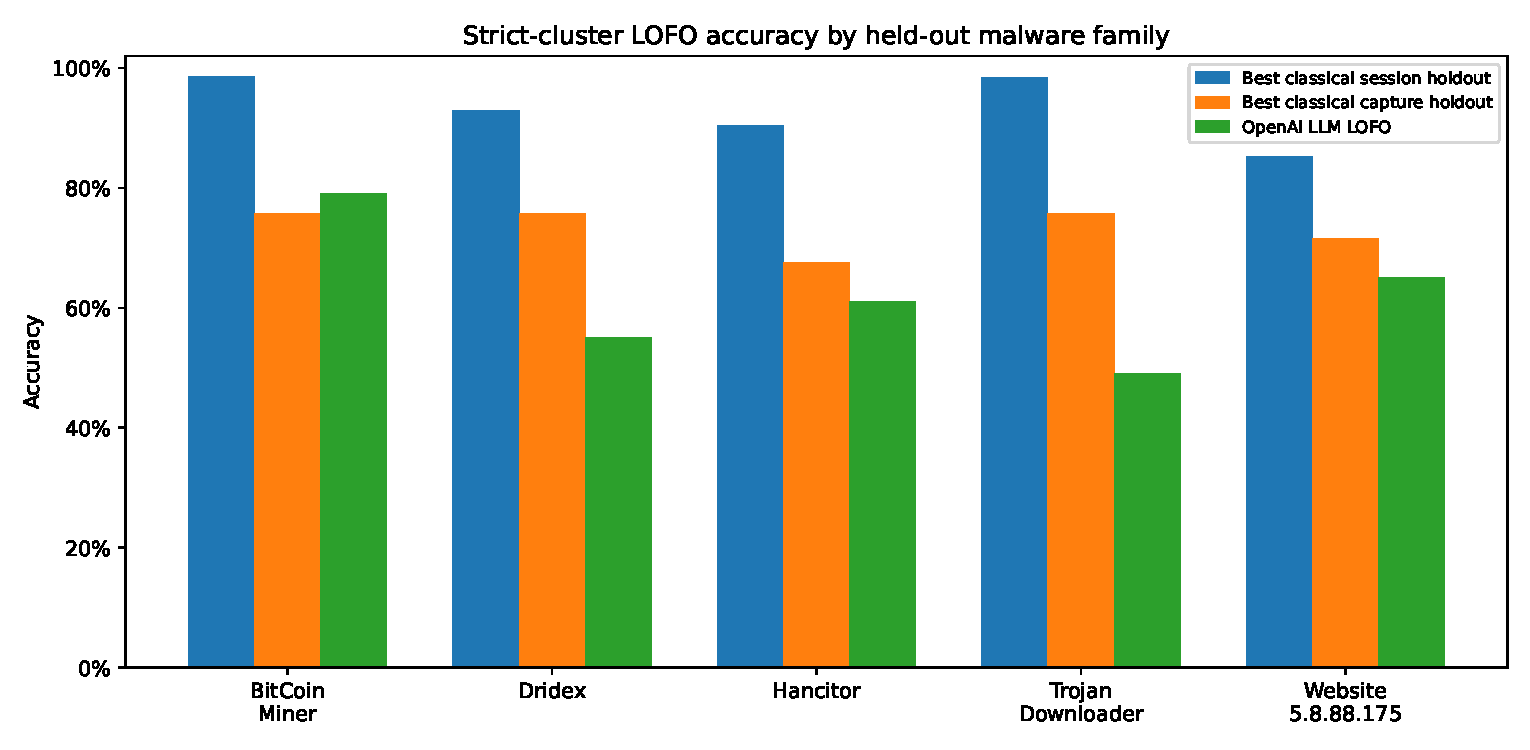
\includegraphics[width=\columnwidth]{lofo_family_comparison.pdf}
\caption{Cluster~1 LOFO accuracy by held-out family. The best session-holdout classical model remains above LLMs for every family.}
\label{fig:lofo-family}
\end{figure}

\subsubsection{Adversarial robustness.}

The adversarial experiments are easier to be read as four separate questions. 
\begin{itemize}
    \item Packet-level evasion asks whether a perturbed malicious packet is relabeled as normal. 
    \item Transfer asks whether a perturbation designed against one model also fools another model without any further modification. Transfer is included because the LLM is treated as a black-box API and does not expose gradients or internal scores for direct white-box optimization. We thus first craft adversarial packets against accessible source models on the same five-feature space, specifically CART and KNN, and then submit those unchanged perturbed feature vectors to the LLM.
    \item Session-level consistency asks whether many individually perturbed packets can overturn the majority verdict of a malicious session.
    \item Black-box search and adaptive query complexity ask whether the LLM can be fooled when the attacker only sees model outputs and must search by repeated API queries.
\end{itemize}

The adversarial section is intended as a representation-space robustness study, because both the classical and LLM detectors consume the same engineered side-channel features. The experiment asks whether bounded, physically plausible changes in the deployed feature representation are enough to change decisions. It does not claim that every successful perturbation is a fully replayable end-to-end packet manipulation under arbitrary application semantics. That position is already compatible with current limitations. Also, the study is a purely isolated-point analysis. The Cluster~1 includes session-level perturbation over 200 perturbed sessions, transfer attacks, black-box search, and adaptive query-complexity analysis. We are careful about distinguishing packet sensitivity from session-level persistence. In that strict setting, packet-level LLM evasion is high, transfer reaches $60–82\%$, and black-box hill-climbing succeeds in $66–82\%$ of cases, but session-level majority detection on perturbed sessions remains $98–99\%$ for the LLM and $91–99\%$ for CART. 

\begin{figure*}[t]
\centering
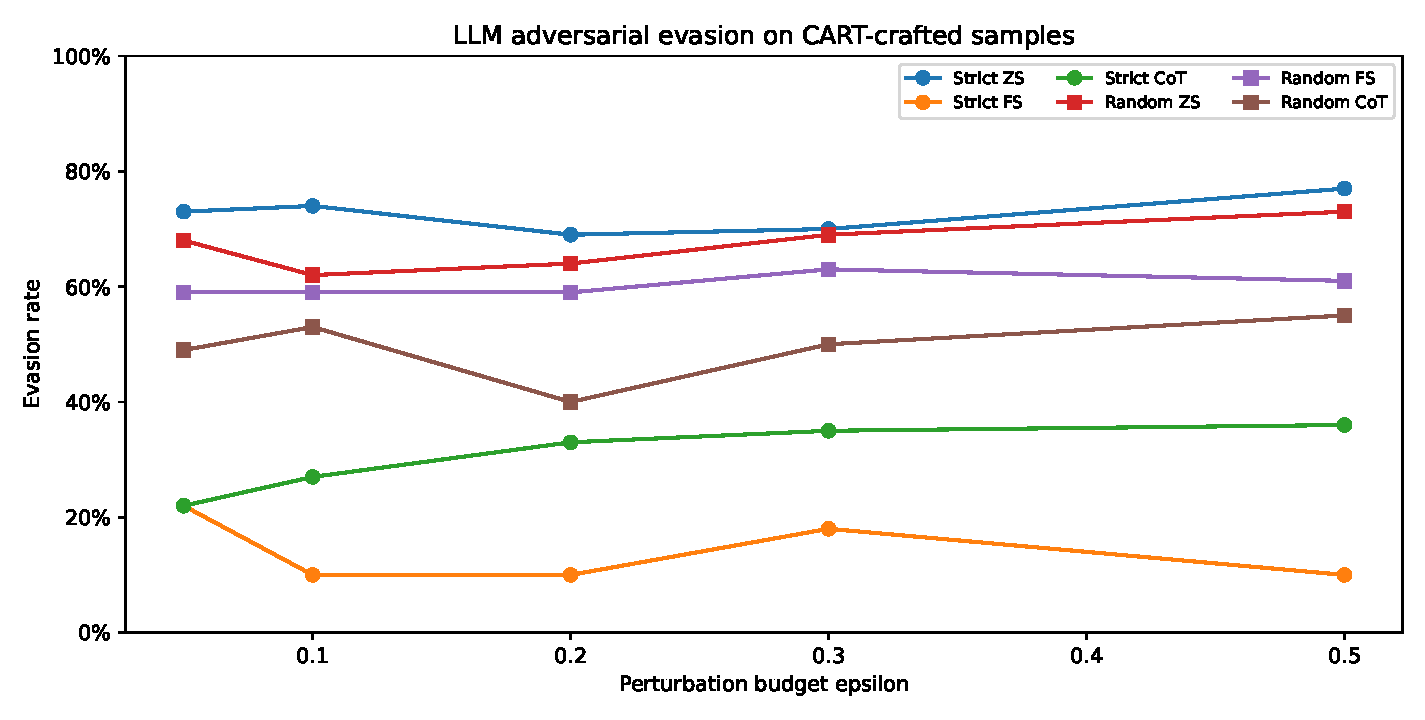
\includegraphics[width=\linewidth]{adversarial_llm_evasion.pdf}
\caption{figure}{LLM evasion on CART-crafted adversarial samples. Zero-shot (ZS) vulnerability is high in both clusters, few-shot prompting helps substantially in Cluster~1 but not enough to close the gap.}
\label{fig:adv-packet-compare}
\end{figure*}

Adversarial evaluation in Cluster~1 covers packet-level evasion, transfer, session-level consistency, black-box search, and adaptive query complexity. Tables~\ref{tab:strict-adv} and ~\ref{tab:strict-tree-ensembles} reports the main packet-level and transfer trends for CART-crafted adversarial samples. Session detection is measured on 100 perturbed sessions; black-box HC denotes hill-climbing evasion against LLMs. CART and KNN packet-level evasion remain in the single digits or low teens, while LLM zero-shot evasion stays between 69\% and 77\%. Few-shot prompting substantially improves LLM robustness on these crafted samples, but evasion still reaches 18\% at $\epsilon=0.30$. Chain-of-thought sits between zero-shot and few-shot. Transfer from CART-crafted samples to the LLM ranges from 60\% to 82\%. On perturbed sessions, however, majority voting remains strong: the LLM session detector stays at 98--99\% across all $\epsilon$ values, slightly above CART at higher budgets. The black-box results are more pessimistic: hill climbing succeeds 66--82\% of the time and random search 84--98\%. Finally, adaptive query-complexity experiments show 95--100\% LLM evasion within a mean of 5.05--7.10 queries and a cost of roughly \$0.015--\$0.021 per successful evasion. Figure \ref{fig:adv-packet-compare} graphically presents these findings showing a clear disadvantage of LLMs against classical algorithms.

\begin{table*}[t]
\centering
\caption{Cluster~1 adversarial summary for CART-crafted samples.}
\label{tab:strict-adv}
\footnotesize
\begin{adjustbox}{width=\textwidth}
\begin{tabular}{ccccccccc}
\toprule
$\epsilon$ & CART evade & KNN evade & LLM ZS evade & LLM FS evade & LLM CoT evade & CART$\rightarrow$LLM transfer & LLM session det. & Black-box HC \\
\midrule
0.05 & 4\%  & 2\% & 73\% & 22\% & 22\% & 62\% & 99\% & 74\% \\
0.10 & 7\%  & 1\% & 74\% & 10\% & 27\% & 60\% & 99\% & 66\% \\
0.20 & 12\% & 4\% & 69\% & 10\% & 33\% & 70\% & 99\% & 82\% \\
0.30 & 9\%  & 1\% & 70\% & 18\% & 35\% & 72\% & 99\% & 82\% \\
0.50 & 9\%  & 1\% & 77\% & 10\% & 36\% & 82\% & 98\% & 78\% \\
\bottomrule
\end{tabular}
\end{adjustbox}
\end{table*}


\subsubsection{Tree-Ensemble models under Cluster~1 Holdout}
\label{subsec:strict-ensembles}

Cluster~1 with compared against results for Tree-Ensemble Baselines, and specifically Random Forest (RF), XGBoost (XGB), and LightGBM (LGBM). These models were trained on the same five-feature representation: packet size, payload size, payload ratio, ratio to the previous packet, and inter-packet time difference. As in the rest of Cluster~1, Experiments~E1--E3 remain packet-level prediction tasks, but train/test separation is enforced at the session or capture level. The presented ensemble runs were executed in a separate phase with independently redrawn packet subsets to be directly comparable to CART/KNN runs at the level of corpus, feature set, and holdout logic.

\begin{table*}[t]
\centering
\caption{Cluster~1 tree-ensemble results. Cell reports accuracy with malicious-class $F_1$ in parentheses. E1 and E2 are mixed-traffic packet tasks under grouped holdout, E3 is encrypted-only, and LOFO columns report macro-averages over five held-out malware families.}
\label{tab:strict-tree-ensembles}
\footnotesize
\resizebox{\textwidth}{!}{%
\begin{tabular}{lcccccccc}
\toprule
Algorithm & E1 Session & E1 Capture & E2 Session & E2 Capture & E3 Session & E3 Capture & LOFO Session Avg. & LOFO Capture Avg. \\
\midrule
RF   & 0.9894 (0.9817) & 0.9764 (0.9625) & 0.9878 (0.9794) & 0.7186 (0.6900) & 0.9944 (0.9070) & 0.9954 (0.8194) & 0.8929 (0.8706) & 0.7195 (0.7665) \\
XGB  & 0.9857 (0.9751) & 0.9695 (0.9508) & 0.9866 (0.9774) & 0.7075 (0.6815) & 0.9930 (0.8829) & 0.9886 (0.4237) & 0.9152 (0.9040) & 0.7260 (0.7770) \\
LGBM & 0.9880 (0.9791) & 0.9706 (0.9527) & 0.9864 (0.9771) & 0.7035 (0.6787) & 0.9939 (0.8979) & 0.9881 (0.4073) & 0.9094 (0.8955) & 0.7095 (0.7607) \\
\bottomrule
\end{tabular}%
}
\end{table*}

Table~\ref{tab:strict-tree-ensembles} shows that RF is the strongest of the newly added ensembles on all six grouped-holdout E1--E3 tasks. On mixed session holdout (E1), RF reaches 98.94\% accuracy with malicious-class $F_1=0.9817$, essentially matching the previously reported CART and KNN results (98.98\% / 0.9827 and 98.91\% / 0.9816, respectively). On the limited 20K session-holdout experiment (E2), all three ensemble methods remain near-saturated, with RF again leading at 98.78\%, followed by XGB at 98.66\% and LGBM at 98.64\%. Because this phase was independently resampled, these small advantages over the earlier CART/KNN session-holdout numbers should be read as corroborating competitiveness rather than as definitive paired wins. On encrypted session holdout (E3), RF again remains very close to the best earlier baselines, but KNN still retains a slight edge (99.46\% accuracy and $F_1=0.9137$ versus 99.44\% and $F_1=0.9070$ for RF).

Capture holdout is more discriminative and reveals a less uniform picture. On E1 mixed capture holdout, RF (97.64\%, $F_1=0.9625$) is effectively tied with CART (97.68\%, $F_1=0.9624$) and only marginally below KNN (97.85\%, $F_1=0.9655$), whereas XGB and LGBM are marginally weaker. The strongest negative result appears in E2 limited capture holdout: RF/XGB/LGBM fall to 71.86\%, 70.75\%, and 70.35\% accuracy, with malicious recall near 0.99 but precision only about 0.53, 0.52, and 0.52, respectively. By contrast, the earlier CART and KNN baselines remain near 98\% on the same experimental template. This indicates that the larger ensemble models can become miscalibrated under low-data, capture-shifted training, aggressively over-predicting the malicious class. Encrypted capture holdout (E3) shows the opposite pattern. Here RF is the winner among the newly added ensembles and also surpasses the earlier CART/KNN baselines, reaching 99.54\% accuracy with malicious-class $F_1=0.8194$, compared with 98.79\% / 0.6048 for KNN and 98.45\% / 0.4775 for CART. XGB and LGBM maintain high overall accuracy in this setting, but their malicious recall collapses to roughly 0.30 and 0.29, yielding much weaker malicious-class $F_1$ values of 0.4237 and 0.4073. This is an important reminder that overall accuracy alone is misleading on highly imbalanced encrypted capture holdout.

The LOFO experiments likewise yield a mixed outcome. Averaged over the five held-out malware families, XGB achieves the best ensemble score under session-group LOFO (91.52\% accuracy, $F_1=0.9040$), slightly above the earlier CART average (91.02\%) but still below KNN (92.78\%). LGBM remains close to CART on average (90.94\%), while RF is pulled down by weaker transfer on Dridex (89.29\% average). Family-wise, the best session-LOFO result across all tested classical models is split across learners rather than monopolized by any one method: LGBM is strongest on BitCoinMiner, RF on Hancitor, KNN on Dridex and Website\_5.8.88.175, and CART on TrojanDownloader. Under the stricter capture-group LOFO, XGB obtains the best ensemble average (72.60\%), but CART still remains the strongest overall model on average (73.28\%) and on four of the five held-out families; the only family for which an ensemble clearly leads is Hancitor, where XGB reaches 73.71\%.



\subsection{Cluster 2: Generic random packet splits with network session leakage}

Cluster~2 is used because it captures a more permissive evaluation style that is still common and more generic. Random packet-level train/test partitioning, no repaired-family LOFO, and an LLM evaluated on a pre-fix database provides insights on whether session-specific data can augment or inhibit detection over minimal characteristics. 

Table~\ref{tab:random-classical} shows that the random packet split does not materially change the headline performance of the strongest classical models on the mixed tasks. KNN and CART again operate at approximately 99\% accuracy on E1 and E2, and above 99.5\% on encrypted traffic. This is an important nuance: for the strongest classical methods the biggest realism penalty does not come from session leakage alone, but from harder settings such as capture holdout and family holdout.

\begin{table*}[t]
\centering

\begin{minipage}[t]{0.60\textwidth}
\centering
\caption{table}{Cluster~2 classical baselines under random packet-level splitting. Each cell reports Accuracy with malicious-class $F_1$ in parentheses.}
\label{tab:random-classical}
\footnotesize
\resizebox{\linewidth}{!}{%
\begin{tabular}{lccc}
\toprule
Algorithm & E1 Random & E2 Random & E3 Encrypted Random \\
\midrule
LR   & 0.7866 (0.5676) & 0.8232 (0.6143) & -- \\
LDA  & 0.8066 (0.5548) & 0.8082 (0.5652) & -- \\
KNN  & 0.9913 (0.9856) & 0.9838 (0.9735) & 0.9958 (0.9369) \\
CART & 0.9901 (0.9834) & 0.9863 (0.9774) & 0.9951 (0.9252) \\
NB   & 0.7026 (0.1100) & 0.6960 (0.1041) & -- \\
SVC  & 0.3015 (0.4608) & 0.8195 (0.6155) & -- \\
MLP  & 0.9630 (0.9374) & 0.9508 (0.9162) & -- \\
\bottomrule
\end{tabular}%
}
\end{minipage}
\hfill
\begin{minipage}[t]{0.37\textwidth}
\centering
\caption{table}{Cluster~2 LLM results. Tokens are total token usage per experiment.}
\label{tab:random-llm}
\footnotesize
\resizebox{\linewidth}{!}{%
\begin{tabular}{lccc}
\toprule
Experiment & Accuracy & $F_1^{\mathrm{mal}}$ & Tokens \\
\midrule
4A zero-shot & 0.6240 & 0.4535 & 207{,}992 \\
4B few-shot $k=1$  & 0.6600 & 0.4848 & 141{,}570 \\
4B few-shot $k=3$  & 0.7000 & 0.5909 & 174{,}053 \\
4B few-shot $k=5$  & 0.5900 & 0.5914 & 209{,}861 \\
4B few-shot $k=10$ & 0.6833 & 0.5455 & 325{,}616 \\
4C chain-of-thought & 0.6450 & 0.5235 & 186{,}532 \\
4E session $w=5$  & 0.6000 & 0.3750 & 167{,}631 \\
4E session $w=10$ & 0.5750 & 0.3089 & 229{,}365 \\
4E session $w=20$ & 0.6300 & 0.4861 & 362{,}098 \\
4E session $w=50$ & 0.5477 & 0.6786 & 738{,}988 \\
\bottomrule
\end{tabular}%
}
\end{minipage}

\end{table*}

\paragraph{Cluster~2 packet prompts and session windows.}
The Cluster~2 experimentation produces somewhat higher packet-level LLM scores than the stricter Cluster~1 run: 62.4\% zero-shot, 70.0\% best few-shot (at $k=3$), and 64.5\% CoT. Those gains do not close the gap to classical ML. The session-window story is again unstable. Accuracy ranges from 57.5\% to 63.0\% for 5--20 bi-directional windows and then drops to 54.8\% at 50 packets. Unlike in Cluster~1, experiment 4E does not record per-call latency, and the cohort is not fixed across window sizes, so the 4E numbers are descriptive rather than controlled.

The adversarial archive still shows high LLM susceptibility on minimal features. For CART-crafted samples, LLM zero-shot evasion stays between 62\% and 73\%, few-shot between 59\% and 63\%, and CoT between 40\% and 55\%. Session-level LLM detection on perturbed sessions remains high (96--99\% for $\epsilon \leq 0.30$ in the saved archive). 

\subsection{Comparative analysis of experimentation clusters}

\begin{table*}[t]
\centering
\caption{High-level comparison between experiment Clusters~1 and ~2.}
\label{tab:cluster-compare}
\footnotesize
\begin{tabularx}{\textwidth}{p{3.2cm}p{3.0cm}p{3.0cm}X}
\toprule
Metric & Cluster~1 strict & Cluster~2 random-leakage & Interpretation \\
\midrule
Split design & Session-group and capture-group holdout & Random 70/30 packet split & Only Cluster~1 supports claims about unseen sessions and unseen captures. \\
LLM provider & OpenAI \texttt{gpt-5.4} & {OpenAI \texttt{gpt-5.4} and Claude Sonnet~4.6} & Cross-cluster differences are confounded by methodology. \\
Packet records & 4{,}656{,}613 & 4{,}692{,}639 & The strict cluster uses revised sessionization and a slightly different packet accounting. \\
Best classical E1 accuracy & 98.98\% (CART session) / 97.85\% (KNN capture) & 99.13\% (KNN) & Leakage has limited effect on the easiest classical mixed-packet task; capture holdout is more informative. \\
Best LLM packet accuracy & 68.0\% (4B $k=10$) & 70.0\% (4B $k=3$) & Both remain far below classical ML. \\
Best LLM session-window accuracy & 96.0\% ($w=5$), then 59.5\%, 50.5\%, 50.0\% & 63.0\% ($w=20$) & Session prompting is unstable and non-monotonic in both clusters. \\
LOFO availability & Yes; overall 61.8\% and best classical session-holdout 82.97--98.62\% & No Cluster~2 LOFO & Family claims come from Cluster~1 only. \\
LLM adversarial vulnerability & ZS 69--77\%, transfer 60--82\%, black-box HC 66--82\% & ZS 62--73\%, deprecated transfer JSON & Both clusters indicate vulnerability; only Cluster~1 supports adversarial conclusions. \\
\bottomrule
\end{tabularx}
\end{table*}

Figures~\ref{fig:adv-packet-compare}, \ref{fig:llm-packet-compare},\ref{fig:llm-session-compare} and Table~\ref{tab:cluster-compare} summarize the relationship between the two clusters. Four comparisons are especially important.

First, the classical picture is stable at the top end. KNN and CART are already so strong on the mixed packet tasks that moving from a random packet split to session-group holdout changes little. The more meaningful realism penalties appear when we hold out entire captures and entire malware families, not merely when we prevent within-session leakage.

Second, the LLM story is more sensitive. Cluster~2 reports higher packet-level LLM scores than Cluster~1, but that difference is affected by split design. Thus, we avoid direct attribution. What is clear in both clusters is that the LLM never approaches the strongest classical baselines on the packet tasks.

Third, session-level prompting is brittle rather than uniformly useless. Cluster~1 run achieves an unusually strong 96.0\% at five packets, but the gain does not survive longer bi-directional windows. Cluster~2 run never produces a comparable peak and is likewise unstable across window sizes. Both clusters reject the simple claim that ``more session context monotonically helps'' on this feature representation.

Fourth, adversarial vulnerability is a shared property. Both clusters show high LLM evasion under minimal-feature perturbations. Cluster~1 supports the stronger claim, because it takes into consideration sessions-per-packet and allows for black-box and query-complexity experiments, but Cluster~2 reports point in the same direction.

\section{Discussion}
\label{sec:discussion}

The two-cluster study supports a strong skeptical conclusion about general-purpose LLMs on minimal traffic side-channel features. The strict cluster does not support a blanket claim that an LLM can never extract useful signal from this representation: the five-packet session window in Cluster~1 is too strong to ignore. What the evidence shows instead is brittleness. When the prediction problem is packet-level, the LLM stays far below classical ML. When very short session context is introduced, the model may sometimes exploit local regularities. But the gain is not stable across longer bi-directional windows, other providers, LOFO, or adversarial conditions.

The random-leakage cluster shows what the same feature representation can look like under a looser and more optimistic protocol. Its packet-level LLM scores are somewhat higher, and this is why it is useful as a contrast. What it cannot do is establish security claims. The absence of valid LOFO, the presence of session leakage, and the deprecated adversarial transfer archive make it unsuitable as the main basis of the paper.

The "rich, raw dataset" hypothesis still explains the main gap. The literature we survey in Section~\ref{sec:related} remains dominated by extensive and detailed datasets with raw bytes, tokenized flows, TLS handshakes, or large statistical summaries. Our five-feature representation removes all of that. What remains is a small numerical classification problem. Cluster~1 shows that the classical models most aligned with that representation --- especially KNN and CART --- remain extremely effective, while the LLM does not display a consistent reasoning advantage. This is what the detailed dataset hypothesis predicts: when byte-level and protocol-level cues disappear, so does most of the apparent LLM advantage reported in richer traffic-analysis settings~\cite{lin2022etbert,cui2025trafficllm,jia2025mentor,ginige2024trafficgpt}.

\subsection{Short vs long context}

The strongest new positive signal in the paper is 4E at $w=5$ in Cluster~1. Short context may help, but long context does not scale. A plausible interpretation is that five packets preserve just enough local temporal patterning to let the model distinguish certain beaconing-like or structured exchanges. That interpretation is still limited, because the effect vanishes as the window grows. Token volume increases from 134{,}582 to 570{,}808 across the 4E settings, latency rises from 2.51 to 4.22 seconds per call, and accuracy collapses. The most likely explanation is that longer minimal-feature sequences dilute the very signal the LLM can weakly exploit at short range. In other words, additional context is not inherently helpful unless the representation itself remains semantically rich enough for the model to reason over it.

\subsection{Penalties, LOFO, and adversarial testing}

Cluster~2 clarifies where evaluation matters most. For the strongest classical baselines, preventing packet leakage alone does not dramatically change E1/E2 headline accuracy, because the task is already easy on the mixed corpus. The real penalties appear in capture holdout and LOFO. Capture-level encrypted testing sharply reduces malicious-class $F_1$, and family holdout separates the classical models from the weaker LLM much more clearly than random packet splits do. Adversarial testing strengthens the same conclusion. Even after parser fixes and invalid-output exclusion, the LLM remains highly permeable to perturbations and to low-query black-box search.

Few-shot prompting helps, but does not solve the problem. Few-shot prompting is not uniformly ineffective. In the strict cluster, few-shot prompts substantially reduce adversarial evasion relative to zero-shot on CART-crafted samples. They also improve clean packet-level accuracy from 50.8\% to 68.0\%. That said, the improvement is not enough. The LLM still remains far below classical ML on clean packet tasks and still highly vulnerable under transfer and black-box attack. 

\section{Limitations}
\label{sec:limitations}

The dataset is a local 12-capture corpus rather than a real-time benchmark, and packet accounting changes after the sessionization. Clusters ~1 and ~2 differ in split design, sessionization, family labeling, and adversarial accounting. Although this is intended to show that LLMs are limited in both session-aware and random packet analysis, we still acknowledge that direct comparison of results is not always coherent and we, thus, use the cross-cluster comparison descriptively, not causally.

\begin{figure}[t]
\centering
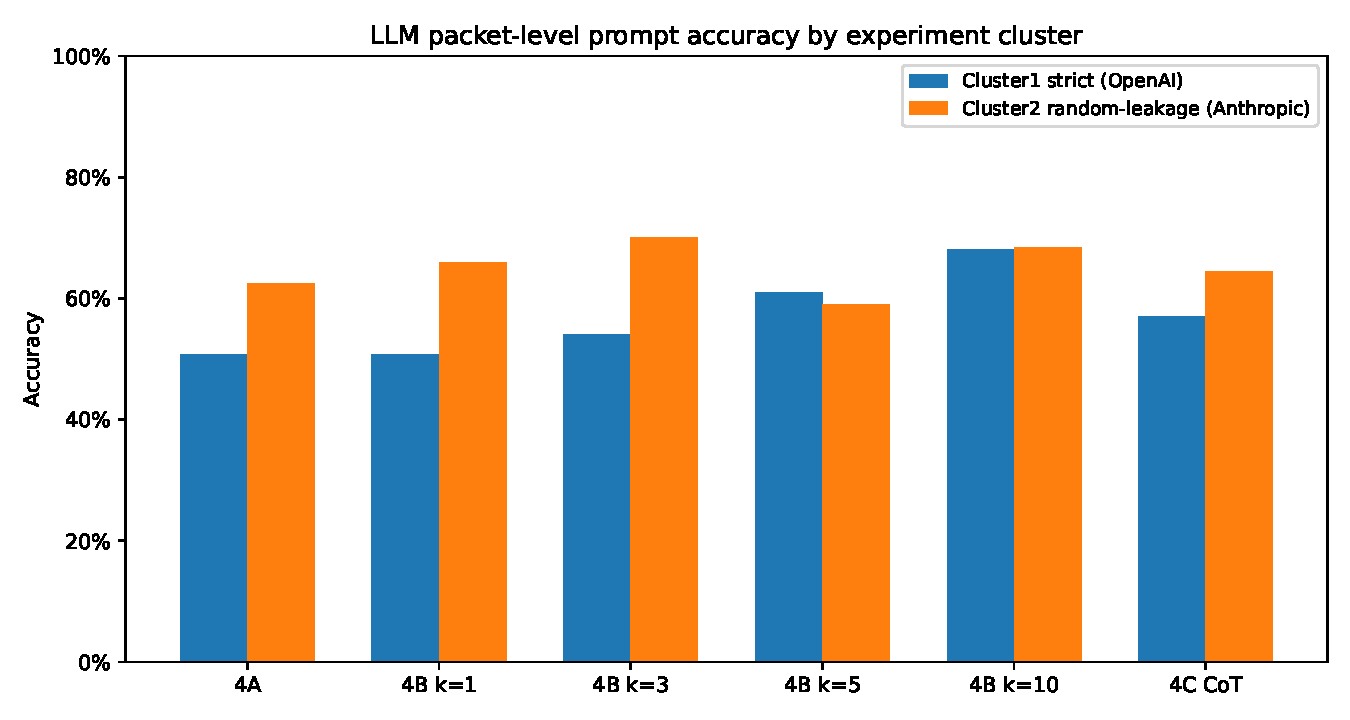
\includegraphics[width=\linewidth]{llm_packet_comparison.pdf}
\caption{Packet-level LLM prompt accuracy by cluster. Cluster~2 yields somewhat higher packet-level scores, but both clusters remain well below classical ML.}
\label{fig:llm-packet-compare}
\end{figure}\hfill
\begin{figure}[t]
\centering
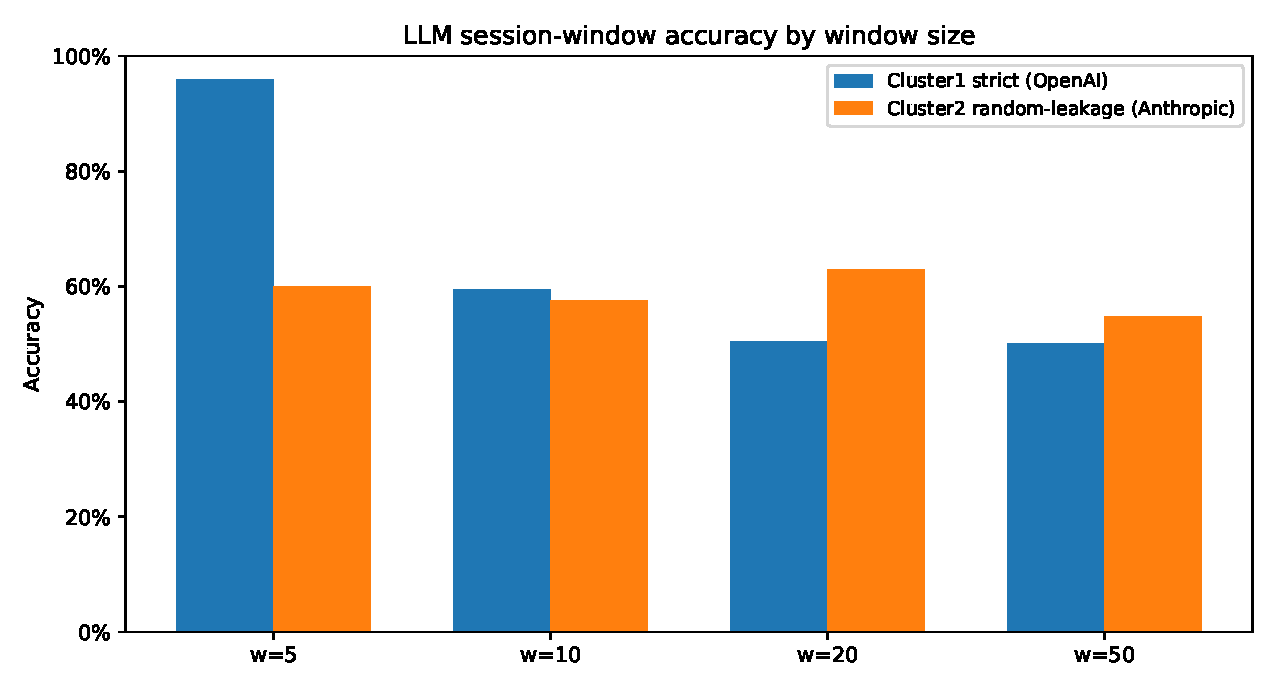
\includegraphics[width=\linewidth]{llm_session_windows.pdf}
\caption{Session-window accuracy by cluster. Cluster~1 peaks at five packets and then collapses, while Cluster~2 remains unstable across all window sizes.}
\label{fig:llm-session-compare}
\end{figure}





Also, even in the strict cluster, classical E1--E3 and LLM 4A--4D are still packet-level decision tasks; only the split unit is session- or capture-aware. Thus the paper evaluates packet classification under realistic holdout plus dedicated session-level analyses, not an end-to-end session classifier throughout. Experiment~4E uses fixed bi-directional windows of length 5--50 rather than random windows. 

Again, this work does not implicitly state that CART/KNN/MLP are the universally optimal NIDS models, nor is it intended as a study for tabular ML. The question is specific to scaling real-time detection through engineered features in network traffic. Once traffic is reduced to  minimal side-channel groups of features, does a generic LLM provide value over representative lightweight conventional classifiers? Our results show that it does not. Several conventional families already dominate the generic LLM by large margins under session- and capture-aware evaluation, so the main conclusion does not depend on proving that these are the absolute best possible classical models.

The LLM API usage is not exhaustively optimized on purpose to argue against work that proposes the use of generic LLMs "as-is" in the context of network intrusion detection. The reported runs use one verbose prompt template family and compare zero-shot, few-shot, and chain-of-thought variants. We do not evaluate domain-specific fine-tuning, retrieval-augmented context, or exhaustive prompt rewriting. 

Lastly, we evaluate one OpenAI model and one Anthropic model, not the full space of general-purpose LLMs. Results could differ quantitatively for different models optimized for numerical reasoning or for different corpus, but the limitation is likely to persist qualitatively.


\section{Conclusion}
\label{sec:conclusion}

This paper presents a two-cluster experiment on minimal five-feature side-channel traffic representations. The primary evidence base is the strict Cluster~1 with session- and capture-group holdout, family LOFO, adversarial accounting, and connection-aware sessionization. Under that protocol, classical KNN, CART and typical RF/XGB algorithms remain the strongest detectors by wide margins on packet-level tasks, family holdout, and most adversarial settings. LLM detection improves modestly with few-shot prompting and shows success on five-packet session windows, but its performance is not stable across longer windows, held-out families, or adversarial evaluation. The Cluster~2 random-leakage experiment produces somewhat higher packet-level LLM scores, but it still cannot support strong conclusions.

Obviously, the evaluation design and configuration of LLMs (windows, corpus, features) can affect what can be legitimately detected using LLMs on minimal traffic features. Still, when the method becomes stricter and the representational features remain minimal, the classical advantage persists and the flexibility of general-purpose LLMs is substantially limited. Future work and real-world implementations should treat packet-level, session-level, and family-level claims separately, and should compare richer and poorer datasets side by side rather than attributing all performance gains to the language model itself.

% \section*{Open Science}
% Artifacts and output JSON for all experiments can be found on the project's repository at:
% \href{https://anonymous.4open.science/r/limits-side_channel_features_intrusion_detection-BF3F/README.md}{[ANONYMIZED LINK]}

\bibliographystyle{IEEEtran}
\bibliography{references}

\section*{Appendix}
\label{appendix}

We provide artifacts to evaluate core claims, namely (i) whether minimal TCP side-channel features are sufficient for malicious-traffic classification, (ii) whether LLM-based classification generalizes under zero-shot and few-shot settings, and (iii) whether LLM-based decisions differ from classical ML baselines under feature-space adversarial perturbations. We provide an anonymous artifact repository for double-blind review:

The repository is accessible through the direct README link [ANONYMIZED FOR SUBMISSION]:
\begin{center}
\url{https://anonymous.4open.science/r/limits-side_channel_features_intrusion_detection-BF3F/README.md}
\end{center}

No username, password, or private credential is required to inspect the repository during review. Reviewers who wish to rerun API-dependent LLM experiments must supply their own API credentials, as described below. All source code, configuration, split definitions, and available result logs are included anonymously.

\paragraph{Artifact inventory.}
The artifacts needed to evaluate the paper are enumerated below.

\begin{enumerate}
    \item \textbf{Documentation.}
    The repository includes a top-level \texttt{README.md} describing the research objective, experiment phases, latest result summaries, and the major implementation changes in the current artifact version. The dependency list is provided in requirements.txt.

    \item \textbf{Experiment orchestration scripts.}
    The top-level script run\_all.py orchestrates the full pipeline. It exposes separate phases for dataset acquisition, feature extraction, local tree-ensemble baselines, classical ML baselines, LLM experiments, analysis/report generation, and adversarial robustness experiments. The script also provides dry-run and compact-prompt modes, allowing reviewers to inspect prompts and execution paths without issuing paid LLM API calls.

    \item \textbf{Configuration files.}
    The directory configs/ contains config.py, which defines the five side-channel features used throughout the paper, namely packet size, payload size, payload ratio, ratio to previous packet, and time difference. It also records dataset registries, malware-family groupings, holdout parameters, LLM experiment parameters, adversarial perturbation budgets, sessionization timeouts, and API-related settings. 

    \item \textbf{Dataset acquisition and preprocessing code.}
    The file src/download\_datasets.py implements acquisition of public malware-traffic captures and labeled flow files where available. The file src/feature\_extraction.py implements extraction of the five side-channel features from packet captures and labeled flow records. The file src/database.py defines the SQLite schema used to store datasets, sessions, packets, and LLM experiment outputs. 

    \item \textbf{Split and benchmark definitions.}
    The directory split\_manifests/ contains frozen JSON manifests for repeated grouped holdout experiments. The manifests specify the packet cohort, group-disjoint train/validation/test partitions, split metadata, and hashes for session-level, capture-level, leave-one-family-out, and smoke-test settings. The file src/splits.py contains the deterministic grouped-split utilities used to generate and materialize these manifests. 

    \item \textbf{Classical ML baselines.}
    The files src/phase2\_local\_ml.py, src/classical\_ml.py, and src/classical\_ml\_v2.py implement the non-LLM baselines. These include, depending on the phase, CART, KNN, logistic regression, linear discriminant analysis, Gaussian naive Bayes, SVC, MLP, random forest, XGBoost, and LightGBM. 

    \item \textbf{LLM experiment code and logs.}
    The file src/llm\_experiments.py implements the LLM-based experiments, including zero-shot classification, few-shot classification, chain-of-thought prompting, leave-one-family-out evaluation, and session-window analysis. The code supports OpenAI and Anthropic-compatible providers through environment variables. 

    \item \textbf{Adversarial robustness artifacts.}
    The adversarial evaluation code is provided in src/adversarial\_experiments.py and src/adversarial/. These files implement feature-space threat models, CART evasion, KNN evasion, black-box search, adaptive adversaries, session perturbation, and adversarial evaluation.  

    \item \textbf{Analysis and paper-table artifacts.}
    The file src/analysis.py generates comparative analysis outputs, while tables.tex contains LaTeX-formatted result tables used to cross-check the quantitative claims in the paper. These artifacts are included to reduce manual transcription ambiguity between the experiment outputs and the paper.

    \item \textbf{Token validation artifact.}
    Script validate\_token\_reduction.py measures the token savings of compact feature formatting relative to verbose natural-language formatting. This script runs offline, does not issue LLM API calls, and supports independent verification of the paper's token-efficiency claims.
\end{enumerate}

The repository includes saved LLM result artifacts, including llm\_results\_openai\_verbose.json, so reviewers can inspect reported metrics and responses without necessarily rerunning API calls. It also includes result artifacts such as phase2\_local\_ml\_results.json and classical\_ml\_results.json, which allow reviewers to compare the reported tables against the saved outputs.The repository adversarial/ contains generated adversarial samples, reasoning or trace files, result summaries such as evasion\_rates.json, blackbox\_results.json, transfer\_results.json, query\_complexity.json, session\_consistency.json, LaTeX tables such as table\_evasion.tex, and generated figures.

\paragraph{Basic execution.}
During double-blind review, the program committee should use only the anonymous URL above. The repository can be inspected directly through the browser. To execute the artifact locally, reviewers can install the dependencies and run selected phases:

\begin{lstlisting}[style=shellstyle_bw]
python -m venv .venv
source .venv/bin/activate
pip install -r requirements.txt
# Dataset acquisition and feature extraction
python run_all.py --phase 0 1 --rebuild-db
# Classical and local ML baselines
python run_all.py --phase 2 3
# Analysis and table generation
python run_all.py --phase 5
# Adversarial generation and classical-only evaluation
python run_all.py --phase 6 --adv-phase generate
\end{lstlisting}

For LLM-dependent experiments, reviewers must set their own provider credential. The artifact does not contain, and intentionally does not provide, any API secret:

\begin{lstlisting}[style=shellstyle_bw]
export OPENAI_API_KEY=<reviewer-provided-key>
python run_all.py --phase 4 --provider openai --compact
\end{lstlisting}

The LLM phase can also be inspected without making API calls:

\begin{lstlisting}[style=shellstyle_bw]
python run_all.py --phase 4 --provider openai --dry-run
\end{lstlisting}

This dry-run mode prints prompts and execution structure, allowing reviewers to audit the prompt design, feature formatting, and experiment wiring without incurring cost or depending on external model availability.

\paragraph{Artifacts not fully shared.}
Several artifacts are intentionally not bundled in full due to (i) size, since many pcaps are publicly available already and their database artifacts are similarily large, (ii) open citation since they are distributed under open licenses for science. Specifically, we omit the following and provide instructions on how to download and install them for execution.

\textbf{Raw packet captures.}
The pipeline uses public malware-traffic sources and, where configured, locally mounted benign and attack PCAPs under paths such as mnt/benign/ and mnt/attack\_pcap/. We do not redistribute these captures in the anonymous repository because raw network traces can be large, may contain network identifiers or operational metadata, and may be subject to upstream dataset licensing or redistribution constraints. Instead, the repository provides scripts, dataset registries, feature-extraction code, malware-family mappings, and frozen split/result artifacts. Readers can audit the methodology and regenerate features from accessible public sources without requiring us to host raw traffic traces inside the double-blind artifact.

\textbf{Generated SQLite database.}
The generated database data/traffic.db is not treated as a required static artifact. It is derived from the acquisition and extraction phases and may be regenerated from the supplied scripts and configuration. This avoids distributing a large processed database containing network-derived metadata while preserving the full transformation logic used to create it.

\textbf{LLM provider credentials and proprietary model weights.}
The artifact does not include OpenAI or Anthropic API keys, nor does it include proprietary LLM weights. These cannot be shared because they are controlled by external providers and are tied to billing and account-specific authorization.

\textbf{Operational malware or exploit payloads.}
The artifact does not include malware binaries, exploit payloads, command-and-control infrastructure, or packet-payload inspection logic. The experiments operate on five numeric side-channel features and do not require deep-packet inspection. 

\paragraph{Reproducibility scope.}
The API-dependent LLM results may vary if rerun with a different provider, model version, account policy, or rate-limit environment. For this reason, we include saved LLM outputs and aggregate JSON result files so that the reported metrics can be audited even if exact LLM replay is not possible during review.

\paragraph{Summary.}
All artifacts needed to evaluate the paper's core methodology are either included in the anonymous repository or can be downloaded from the official public sources for CTU and Hakari datasets. The only omitted artifacts are raw traffic captures, generated databases, proprietary LLM credentials or weights, and operational malicious payloads.

\end{document}
